\documentclass[11pt]{article}
\usepackage{fullpage,url}
\usepackage{amsmath,amsthm,amssymb}
\usepackage{graphicx}
\usepackage{eso-pic}
\usepackage{bm}
\usepackage{caption}
\usepackage{picins}   
\usepackage{microtype}
\usepackage{multirow}
\usepackage{url}
\usepackage{enumerate}

\usepackage[letterpaper,top=1in,bottom=1in,left=1in,right=1in,nohead]{geometry}

\newenvironment{claim}[1]{\noindent\underline{{\bf Claim:}}\space#1}{}
\newenvironment{claimproof}[1]{\par\noindent\underline{{\bf Proof:}}\space#1}
{\hfill$\square$}

\makeatletter
\newcommand{\specialnumber}[1]{%
  \def\tagform@##1{\maketag@@@{(\ignorespaces##1\unskip\@@italiccorr#1)}}%
}

\setlength{\parindent}{0in}
\setlength{\parskip}{6pt}

\DeclareMathOperator{\E}{E}
\DeclareMathOperator{\Var}{Var}
\DeclareMathOperator{\Unif}{Unif}

\begin{document}
\thispagestyle{empty}
{\large{\bf CS6957: Probabilistic Modeling \hfill Prateep Mukherjee(u0876583)}}\\

{\LARGE{\bf Homework 1}}
\vspace{0.2\baselineskip}
\hrule

1. (a)  First, we use the identity $\int p(x) dx = 1$.

\begin{eqnarray}
 & \int p(x|\eta) dx = 1 \notag \\
& \implies \int h(x) \exp(\eta T(x) - A(\eta)) dx = 1
\label{eq1}
\end{eqnarray}

\par Next, we differentiate Eq. \ref{eq1} w.r.t. $\eta$.
\vspace{-8pt}

\begin{eqnarray}
  \frac{d}{d\eta}  \int h(x) \exp(\eta T(x) - A(\eta)) dx = \frac{d}{d\eta} (1) &=& 0 \notag \\
\implies \int h(x) \; \exp(\eta T(x) - A(\eta)) \; (T(x) - \nabla A(\eta)) dx &=& 0 \notag \\
 \implies \int h(x) \exp(\eta T(x) - A(\eta)) T(x) dx  \notag - \int h(x) \exp(\eta T(x) - A(\eta)) \nabla A(\eta) dx &=& 0  \notag \\
\implies \int p(x|\eta) T(x) dx - \left [ \int p(x|\eta) dx\right ] \nabla A(\eta) &=& 0 \notag \\
\implies E[T(X) | \eta]  &=& \nabla A(\eta) \notag
\end{eqnarray}

Therefore, $E[T(X| \eta)] = \nabla A(\eta) = \left ( \frac{\partial A}{\partial \eta_1}, \frac{\partial A}{\partial \eta_2} \cdots \frac{\partial A}{\partial \eta_d}\right ) $

\par (b) 

\begin{eqnarray*}
  \frac{1}{\sqrt{2\pi}\sigma} \exp(-\frac{(x-\mu)^2}{2\sigma^2}) &=
       \frac{1}{\sqrt{2\pi}\sigma} \exp(-\frac{x^2}{2\sigma^2}) \cdot \exp(\mu \cdot \frac{x}{\sigma^2} - \frac{\mu^2}{2\sigma^2}) \\
&= \frac{1}{\sqrt{2\pi}\sigma} \exp(-\frac{x^2}{2\sigma^2}) \cdot \exp(\eta T(x) - A(\eta))
\end{eqnarray*}

where, $\eta = \frac{\mu}{\sigma^2}$, $A(\eta) = \frac{\mu^2}{2\sigma^2} = \frac{\sigma^2 \eta^2}{2}$, $T(x) = x$ and $h(x) =  \frac{1}{\sqrt{2\pi}\sigma} \exp(-\frac{x^2}{2\sigma^2})$.

\par Thus, we get $E[T(X|\eta)] = E[X|\eta] = \nabla A(\eta) = \eta\sigma^2 = \mu$

\par 2. (a)  The pmf $p(X=k;\lambda)$ is

\vspace{-8pt}
\begin{eqnarray*}
   p(X=k; \lambda) &=& \frac{\lambda^k e^{-\lambda}}{k!} \\
&=& \frac{1}{k!} \cdot \exp( \ln \lambda^k) \cdot e^{-\lambda} \\
&=& \frac{1}{k!} \cdot \exp(-\lambda + \ln \lambda^k) \\
&=& \frac{1}{k!} \cdot \exp(\eta T(x) - A(\eta) )
\end{eqnarray*}

where, natural parameter $\eta = \ln \lambda$, sufficient statistic $T(x=k) = k$ and normalizing constant $A(\eta) = \lambda$.

\par (b)  Two options for non-informative priors(probability mass functions) for $p(\lambda)$ are:
\begin{itemize}
 \item Uniform prior $\rightarrow \lambda \sim Unif(0,1), p(\lambda) = 1$
 \item Jeffrey's prior $\rightarrow p(\lambda) \propto \sqrt{ \frac{1}{\lambda} }$
\end{itemize}

\par (c) Let, $X=(x_1,x_2,\cdots x_n)$ be $n$ observed values for x. Therefore, the posterior distribution for $\lambda$ can be written as:

\vspace{-10pt}
\begin{equation*}
  p(\lambda | x_1, \cdots, x_n) \propto L(\lambda; x_1, x_2, \cdots x_n) \; p(\lambda) 
\end{equation*}

where, $L(\lambda; x_1, x_2, \cdots x_n)$ is the joint likelihood of the observed data. Considering that the data is i.i.d. and the uniform prior $p(\lambda) \propto 1$, we can write the following:

\vspace{-20pt}
\begin{eqnarray}
  p(\lambda | x_1, \cdots, x_n) &\propto& \prod_{k=1}^{n} p(x_k | \lambda) \; p(\lambda)  \notag \\
&\propto& \prod_{k=1}^{n} \frac{\lambda^{x_k}e^{-\lambda}}{x_{k}!} \cdot 1 \notag  \\
&\propto& \prod_{k=1}^{n} \lambda^{x_k} e^{-\lambda} \notag \\
&\propto& e^{-n\lambda} \lambda^{\bar{X}+1-1} 
\label{eq2c}
\end{eqnarray}

where, $\bar{X} = \sum\limits_{k=1}^{n} x_k$.  Similarly considering Jeffrey's prior, we get
\vspace{-10pt}
\begin{equation}
  p(\lambda | x_1, \cdots, x_n) \propto  e^{-n\lambda} \lambda^{\bar{X}+1/2-1} 
\label{eq2c1}
\end{equation}

Eqs. \ref{eq2c},\ref{eq2c1} are the \emph{Gamma} distributions. Therefore, the posterior distributions for $\lambda$ are

\begin{equation*}
  p(\lambda | X) = 
\begin{cases}
   Gamma(\lambda; \bar{X}+1, n), \; \; \; \; \; \; \; \; \; \; \; \;  \mbox{$p(\lambda) \sim Unif$} \\
    Gamma(\lambda; \bar{X}+1/2, n), \; \; \; \; \; \; \; \; \mbox{$p(\lambda) \sim Jeff$}
\end{cases}
\end{equation*}
\vspace{-10pt}
where $\Gamma(n) = (n-1)!$. The \emph{Gamma} distribution is defined as :

\vspace{-10pt}
\begin{equation}
Gamma(x; a,b) = \frac{a^b}{\Gamma(a)} \cdot x^{a-1} \cdot \exp(-bx)
\label{eq2c2}
\end{equation}

To compute whether $p(\lambda | X)$ is proper or improper, we have to show that $\sum\limits_{\lambda} p(\lambda | X) = 1$.  For the uniform prior,

\vspace{-20pt}
\begin{eqnarray}
\sum\limits_{\lambda=0}^{\infty} p(\lambda | X) &=& \sum\limits_{\lambda=0}^{\infty} \frac{n^{\bar{X}+1}}{\Gamma(\bar{X}+1)} \cdot \left [ \lambda^{\bar{X}} \cdot \exp(-n\lambda) \right ] \notag \\
&=& \frac{n^{\bar{X}+1}}{\Gamma(\bar{X}+1)} \cdot \left [ \sum\limits_{\lambda=0}^{\infty} \lambda^{\bar{X}} \cdot \exp(-n\lambda) \right ] \notag \\
&=& \frac{n^{\bar{X}+1}}{(\bar{X})!} \cdot \Gamma(\bar{X}+1) \notag \\
&=& \frac{n^{\bar{X}+1}}{(\bar{X})!} \cdot (\bar{X})!  = n^{\bar{X}+1} 
\label{eq2c3}
\end{eqnarray}

Similarly, using Jeffrey's prior, we get $\sum\limits_{\lambda=0}^{\infty} p(\lambda | X) = n^{\bar{X}+1/2}$. This and eq. \ref{eq2c3} are both finite. Therefore, the posterior distribution for both Uniform and Jeffrey's prior are proper. 

\par 3. The pdf for $\mu$ is,

\begin{equation*}
p(\mu) = 
\begin{cases}
  \frac{1}{b-a}, \; \; \; \; \; \; \; \; \mbox{if $a \le \mu \le b$}, \\
  0, \; \; \; \; \; \; \; \; \; \; \; \; \mbox{otherwise}
\end{cases}
\end{equation*}

According to Bayes' rule,

\begin{equation*}
  p(\mu | x_1, \cdots, x_n) = \frac{p(x_1, \cdots, x_n | \mu)p(\mu)}{\int_{\mu} p(x_1, \cdots, x_n, \mu) d\mu}
\end{equation*}

Since $p(\mu) = 0$, when $ \mu \notin [a,b]$, we can modify the bounds of the integral. Thus, posterior pdf 

\begin{eqnarray*}
  p(\mu | x_1, \cdots, x_n; \sigma^2,a,b) &=& \frac{ \left [ \prod\limits_{i=1}^n p(x_i|\mu,\sigma^2) \right] \cdot p(\mu|a,b) } {\int\limits_{\mu=a}^{\mu=b} \left [ \prod\limits_{i=1}^{n} p(x_i|\mu,\sigma^2)\right] \cdot p(\mu|a,b) d\mu } \\
  &=& \frac{ \left[ \frac{1}{(\sqrt{2\pi} \sigma)^n} \exp(-\sum\limits_{i=1}^{n} \frac{(x_i-\mu)^2}{2\sigma^2}) \right] \cdot \frac{1}{b-a} }{ \int\limits_{\mu=a}^{\mu=b}\left[ \frac{1}{(\sqrt{2\pi} \sigma)^n}  \exp(-\sum\limits_{i=1}^{n} \frac{(x_i-\mu)^2}{2\sigma^2}) \right] \cdot \frac{1}{b-a} d\mu} \\
&=& \frac{ \exp(-\sum\limits_{i=1}^{n} \frac{(x_i-\mu)^2}{2\sigma^2}) }{\int\limits_{\mu=a}^{\mu=b} \exp(-\sum\limits_{i=1}^{n} \frac{(x_i-\mu)^2}{2\sigma^2}) d\mu} \\
&=& \frac{\exp(-\frac{n\mu^2-2n\bar{x}\mu}{2\sigma^2} )}{\int\limits_{\mu=a}^{\mu=b} \exp(-\frac{n\mu^2-2n\bar{x}\mu}{2\sigma^2} ) d\mu}, \; \; \; \; \; \; \; \; \;\mbox{(where $\bar{x} = \frac{1}{n} \sum\limits_{i=1}^{n} x_i $)} 
\end{eqnarray*}

\par 4. (a) The joint posterior $p(\mu_j, \sigma^{2}_{j} | y_{ij})$ is a normal inverse gamma distribution.

\begin{equation*}
	p(\mu_j, \sigma^{2}_{j} | y_{ij})  = NIG(\mu_{n}, n_{n}, \alpha_{n}, \beta_{n}),
\end{equation*}
where,
\begin{eqnarray}
  \mu_{nj} &=& \frac{n_0 \mu_0 + n_j \bar{y}_j }{ n_0 + n_j} \notag \\
  n_{nj} &=& n_0 + n_j \notag \\
  \alpha_{nj}  &=& \alpha_0 + \frac{n_{j}}{2} \label{eq4a} \\
  \beta_{nj} &=& \beta_0 + \frac{1}{2} \sum\limits_{i=1}^{n} (y_{ij} - \bar{y}_{j})^2 + \frac{n_j n_0}{n_j + n_0} \frac{(\bar{y}_{j} - \mu_0)^2}{2} \notag
\end{eqnarray}

\par The marginal posterior $p(\sigma_{j}^{2} | y_{ij})$ is an Inverse-Gamma(\emph{IG}) distribution with shape parameter as $\alpha_n$ and scale parameter as $\beta_n$. 

\par I used the \textbf{``LaplacesDemon'' }(\url{http://www.bayesian-inference.com/softwaredownload}) R package for the inverse-gamma and students-t distribtutions.

\begin{figure}[!hbt]
 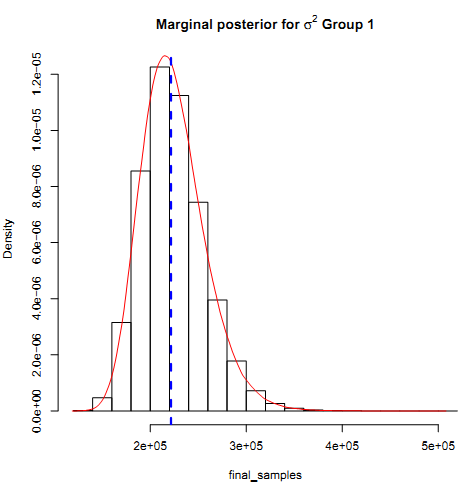
\includegraphics[width=0.5\linewidth] {img4a.png} 
 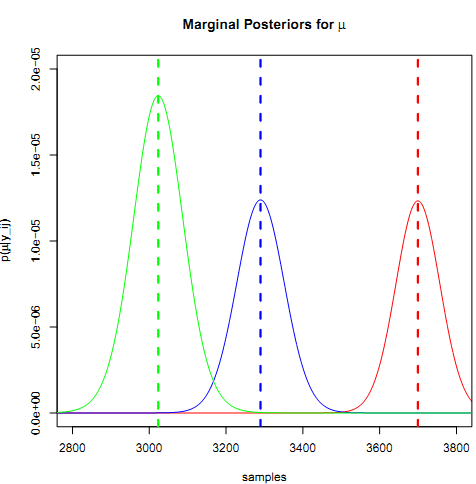
\includegraphics[width=0.5\linewidth] {img4b.png} 
\caption{\small{ {\bf (a):} Marginal posterior $p(\sigma^{2}_{1} | y_{ij})$. Dotted line shows the sample variance of the control group. {\bf (b)} Marginal posterior $p(\mu_{j} | y_{ij})$. Control group is denoted by \textcolor{red}{red}, mild is denoted by \textcolor{blue}{blue} and dementia group is denoted by \textcolor{green}{green}. Dotted lines denote the sample mean respectively. }}
\label{fig4ab}
\end{figure}
\vspace{-10pt}
\par (b) The marginal posterior $p(\mu_{j} | y_{ij})$ is a students-t distribution. 

\begin{equation}
 p(\mu_{j} | y_{ij}) = t(\mu_{j} | \nu = 2\alpha_{nj}, \mu = \sqrt{ \frac{2\beta_{nj}}{n_{nj}} })
\label{eq4b}
\end{equation}

where, $\beta_{nj}$ and $n_{nj}$ are the posterior parameters from eq.\ref{eq4a}. In eq. \ref{eq4b}, $\nu$ denotes the degrees of freedom and $\mu$ denotes the \emph{non-centrality parameter}. Fig. \ref{fig4ab}(b) shows the marginal posterior for the three groups. 

\par (c) The conditional distribution $p(d_{12} | \sigma^{2}_{1}, \sigma^{2}_{2}, y_{ij})$ is a normal distribution, with mean as $\bar{y}_{1} - \bar{y}_{2}$ and variance as ($\frac{\sigma^{2}_{n_1}}{n_1}  + \frac{\sigma^{2}_{n_2}}{n_2}$), where $\sigma^{2}_{n_1}$ and $\sigma^{2}_{n_2}$ are sampled from the posterior distributions $p(\sigma^{2}_{n_1} | y_{i1})$ and $p(\sigma^{2}_{n_2} | y_{i2})$ obtained in (a). The other distributions $p(d_{23} | \sigma^{2}_{2}, \sigma^{2}_{3}, y_{ij})$ and $p(d_{13} | \sigma^{1}_{1}, \sigma^{2}_{3}, y_{ij})$ are obtained similarly.  

\par Probabilities $P(d_{12} < 0 | y_{ij})$ , $P(d_{13} < 0 | y_{ij})$ and $P(d_{23} < 0 | y_{ij})$ are $2*10^{-6}$, $5 * 10^{-6}$ and 0.03. These probabilities tell us that the mild and dementia groups overlap, as shown in Fig. \ref{fig4ab}, by $3\%$. On the other hand, the control group is quite separated from the other groups, using the NIG prior.

\par (d) Using the one-sided t-test with ``less'' as the null hypothesis, we get the highest p-value for $d_{23}$ followed by $d_{13}$ and $d_{12}$. This complies with our analysis that groups mild and dementia actually overlap. The p-value obtained from the t-test denotes the probability that the \emph{alternative} hypothesis holds true. Thus, higher the p-value the event described in the alternative hypothesis  is more likely. In this case, ``less'' denotes the random event $\mu_1 - \mu_2 < 0$. Therefore, highest p-value of $d_{23}$ denotes that this event is most likely. 

% TODO : Write little abt t-test

\par 5. (a) Using Jeffrey's non-informative prior $p(\mu, \sigma^{2} | y_{ij}) \propto \frac{1}{\sigma^2}$, the joint posterior $p(\mu_j, \sigma^{2}_{j} | y_{ij})$ is a normal distribution.

The marginal posterior $p(\sigma^{2}_{j} | y_{ij})$ is a scaled Inv-$\chi^2$ distribution, with parameters $\nu$(degrees of freedom) as $2\alpha_{nj}-1$ and scale parameter is $\bar{\sigma^2_{j}}$, the sample variance for group $j$.

\begin{figure}[!hbt]
 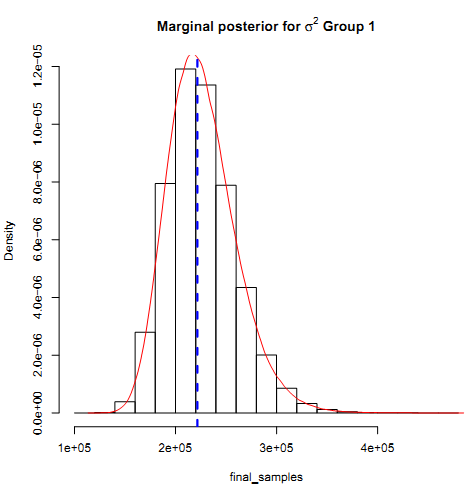
\includegraphics[width=0.5\linewidth] {img5a.png} 
 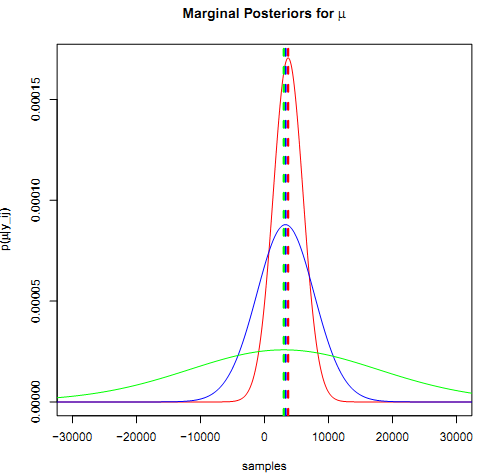
\includegraphics[width=0.5\linewidth] {img5b.png} 
\caption{\small{ {\bf (a):} Marginal posterior $p(\sigma^{2}_{1} | y_{ij})$. Dotted line shows the sample variance of the control group. {\bf (b)} Marginal posterior $p(\mu_{j} | y_{ij})$. Control group is denoted by \textcolor{red}{red}, mild is denoted by \textcolor{blue}{blue} and dementia group is denoted by \textcolor{green}{green}. Dotted lines denote the sample mean respectively. }}
\label{fig5ab}
\end{figure}
\vspace{-10pt}

\par (b) The marginal posterior $p(\mu_{j} | y_{ij})$ is a non-central students' t-distribution with parameters - degrees of freedom($\nu = n_j$) and \emph{non-centrality parameter}(ncp = $\frac{\bar{\sigma^2_{j}}}{n_j}$). The plot of the marginal distributions for the three groups are shown in Fig. \ref{fig5ab}(b).

\par (c) The conditional distribution $p(d_{12} | \sigma^{2}_{1}, \sigma^{2}_{2}, y_{ij})$ is a normal distribution, with mean as $\bar{y_{1}} - \bar{y_{2}}$ and variance as ($\frac{\bar{\sigma^{2}_{n_1}}}{n_1}  + \frac{\bar{\sigma^{2}_{n_2}}}{n_2}$), where $\bar{\sigma^{2}_{n_1}}$ and $\bar{\sigma^{2}_{n_2}}$ are the sample variances of groups 1 and 2 respectively. The other distributions $p(d_{23} | \sigma^{2}_{2}, \sigma^{2}_{3}, y_{ij})$ and $p(d_{13} | \sigma^{1}_{1}, \sigma^{2}_{3}, y_{ij})$ are obtained similarly.  

\par Probabilities $P(d_{12} < 0 | y_{ij})$ , $P(d_{13} < 0 | y_{ij})$ and $P(d_{23} < 0 | y_{ij})$ are $10^{-6}$, $1.5 * 10^{-5}$ and 0.034. 


\par 6. (a,b) Using the given ``pseudo-observations'', we get the following values of the initial parameters: $\mu_0  = 2133, \nu_0 = 127, \sigma_0 = 279, \alpha_0 = n_0/2$ and $\beta_0 = \frac{n_0-1}{2} \sigma^{2}_0$. We use these values for all three groups. Using these values, the joint posterior $p(\mu_j, \sigma^{2}_j | y_{ij})$ for each group $j$ is a NIG distribution, whose parameters are same as those in eq. \ref{eq4a}. 

\par The marginal posterior $p(\sigma^{2}_j | y_{ij})$ is an \emph{Inverse-Gamma} distribution, while $p(\mu_j | y_{ij})$ is a \emph{students-t distribution}, with similar posterior hyperparameters as in 4.

\par Fig \ref{fig6ab} shows the marginal posterior distributions on $\sigma^2$ and $\mu$.

\begin{figure}[t]
 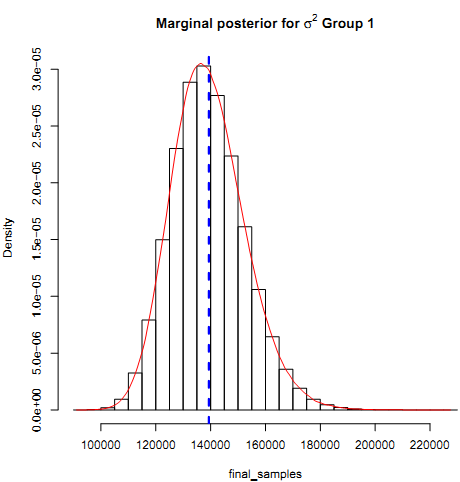
\includegraphics[width=0.5\linewidth] {img6a.png} 
 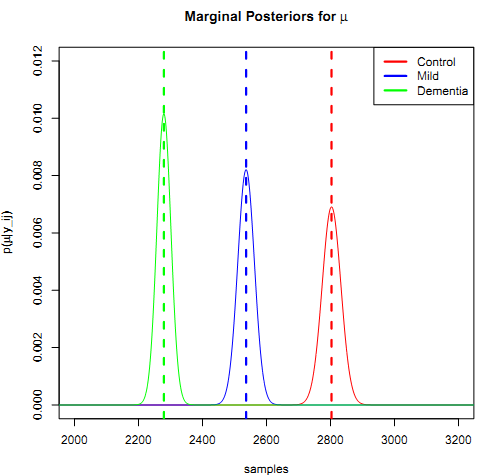
\includegraphics[width=0.5\linewidth] {img6b.png} 
\caption{\small{ {\bf (a):} Marginal posterior $p(\sigma^{2}_{1} | y_{ij})$. Dotted line shows the sample variance of the control group. {\bf (b)} Marginal posterior $p(\mu_{j} | y_{ij})$. Control group is denoted by \textcolor{red}{red}, mild is denoted by \textcolor{blue}{blue} and dementia group is denoted by \textcolor{green}{green}. Dotted lines denote the sample mean respectively. }}
\label{fig6ab}
\end{figure}

\par (c) $P(d_{12} < 0 | y_{ij}), P(d_{13} < 0 | y_{ij})$ and $P(d_{23} < 0 | y_{ij})$ are now 0.0003, 0 and 0.0183 respectively. From Fig. \ref{fig6ab}(b), it can be seen that the peaks are well-separated. Thus, the NIG conjugate prior based on the ``pseudo-observations'' actually help to separate the resulting posteriors of the three groups. 

\par Thus, in this case, prior domain knowledge of the hippocampus data will result in better classification. 

\end{document}